\section*{Supplementary Material}

\subsection*{Derivation of G(r,t)}

\subsubsection*{Diffusion and birth/death processes}

In this section, we aim to find back Eq.~2 in \cite{young_reproductive_2001}, i.e. Eq.~\ref{eq:eq_2_Young_total} in our manuscript. We will first focus on the diffusion and birth/death processes, that is:

\begin{equation}
 \frac{\partial G}{\partial t}=2Dr^{1-d}\frac{\partial}{\partial r}\left(r^{d-1}\frac{\partial G}{\partial r}\right)+2(\lambda-\mu)G+2\lambda C\delta(\boldsymbol{x})\label{eq:eq_2_Young_diffusionbirth}
\end{equation}

\vspace{1.25em}

We first define an ensemble of $k$ identical brownian bugs in a d-dimension
space. The
bug number $p$ is located at $\boldsymbol{x}_{p}=[x_1,x_2,...x_{d}]$.
At time $t$, the space is defined by (a) the number of brownian
bugs $k$ and (b) the vector of their locations $\boldsymbol{X}_{k}=[\boldsymbol{x}_{1},\boldsymbol{x}_{2},...\boldsymbol{x}_{k}]$.
This is also called the Fock space \citep{birch_master_2006}. \\

The probability distribution over
the state space is given by the functions $\mathcal{P}_{k}(\boldsymbol{X}_{k},t)$
such that:

\begin{equation}
\mathcal{P}_{k}(\boldsymbol{X}_{k},t)d\boldsymbol{X}_{k}=\text{Pr}\{k\text{ bugs, with a bug in }d\boldsymbol{x}_{1},\text{a bug in }d\boldsymbol{x}_{2}\text{, etc.}\}
\end{equation}

\vspace{1.25em}

As bugs are indistinguishable, we can exchange $\boldsymbol{x}_{p}$
and $\boldsymbol{x}_{q}$ (permutation symmetry):

\begin{equation}
\mathcal{P}_{k}(\boldsymbol{x}_{1},\ldots,\boldsymbol{x}_{p},\ldots,\boldsymbol{x}_{q},\ldots,\boldsymbol{x}_{k},t)=\mathcal{P}_{k}(\boldsymbol{x}_{1},\ldots,\boldsymbol{x}_{q},\ldots,\boldsymbol{x}_{p},\ldots,\boldsymbol{x}_{k},t)
\end{equation}

\vspace{1.25em}

The normalization is: 

\begin{equation}
\mathcal{P}_{0}(t)+\int\mathcal{P}_{1}(\boldsymbol{X}_{1},t)d\boldsymbol{x}_{1}+\int\int\mathcal{P}_{2}(\boldsymbol{X}_{1},t)d\boldsymbol{x}_{1}d\boldsymbol{x}_{2}+\ldots+\int_{\mathbb{R}^{2k}}\mathcal{P}_{k}(\boldsymbol{X}_{k},t)d\boldsymbol{X}_{k}+\ldots=1
\end{equation}

\vspace{1.25em}

We define $b_{k}(\boldsymbol{x},t)=\int\mathcal{P}_{k}(\boldsymbol{x},\boldsymbol{X}_{k-1},t)d\boldsymbol{X}_{k-1}$, i.e. $b_{k}(\boldsymbol{x},t)d\boldsymbol{x}$ is 
the probability that there are $k$ bugs and bug number 1 is in $d\boldsymbol{x}$.\\

The density of points is defined as:

\begin{equation}
\rho(\boldsymbol{x},t)=\sum_{k=1}^{\infty}kb_{k}(\boldsymbol{x},t)=\sum_{k=1}^{\infty}k\int\mathcal{P}_{k}(\boldsymbol{x},\boldsymbol{X}_{k-1},t)d\boldsymbol{X}_{k-1}
\end{equation}

The pair correlation function is then:

\begin{equation}
G(\boldsymbol{x},\boldsymbol{y},t)=\sum_{k=2}^{\infty}k(k-1)\int\mathcal{P}_{k}(\boldsymbol{x},\boldsymbol{y},\boldsymbol{X}_{k-2},t)d\boldsymbol{X}_{k-2} \label{eq:def_pairdens}
\end{equation}

We define the two particle distribution functions $c_{k}(\boldsymbol{x},\boldsymbol{y},t)=\int\mathcal{P}_{k}(\boldsymbol{x},\boldsymbol{y},\boldsymbol{X}_{k-2},t)d\boldsymbol{X}_{k-2}$. Note that $G(\boldsymbol{x},\boldsymbol{y},t)=\sum_{k=2}^{\infty}k(k-1)c_{k}(\boldsymbol{x},\boldsymbol{y},t)$.\\

\textbf{\underline{Proposition}}\\

The time derivative of $c_k$ is given by:

\begin{subequations} 
\begin{align}
\frac{\partial c_{k}}{\partial t}(\boldsymbol{x},\boldsymbol{y},t) & =D\nabla_{2}^{2}c_{k}\label{ck_diffusion-1}\\
 & -k(\lambda+\mu)c_{k}\label{ck_same_state-1}\\
 & +(k+1)\mu c_{k+1}\label{ck_death-1}\\
 & +2\frac{\lambda}{k}\delta(\boldsymbol{x}-\boldsymbol{y})b_{k-1}(\boldsymbol{x})+\lambda\frac{(k-2)(k+1)}{k}c_{k-1}\label{ck_birth-1}
\end{align}
\end{subequations}

\newpage

\textbf{\underline{Proof}}\\

We write the evolution of $\mathcal{P}_{k}(\boldsymbol{X}_{k},t)$:

\begin{subequations} 
\begin{align}
\frac{\partial\mathcal{P}_{k}}{\partial t} & =D\nabla_{k}^{2}\mathcal{P}_{k}\label{pk_diffusion}\\
 & -k(\lambda+\mu)\mathcal{P}_{k}\label{pk_same_state}\\
 & +(k+1)\mu\int\mathcal{P}_{k+1}(\boldsymbol{X}_{k},\boldsymbol{y},t)d\boldsymbol{y}\label{pk_death}\\
 & +\frac{\lambda}{k}\sum_{p=1}^{k}\sum_{q=1,q\neq p}^{k}\delta({\boldsymbol{x}_p-\boldsymbol{x}_q})\mathcal{P}_{k-1}(\boldsymbol{X}_{k|p,t})\label{pk_birth}
\end{align}
\end{subequations}

where $\nabla_{k}^{2}=\frac{\partial^{2}}{\partial_{x_{1}}^{2}}+\frac{\partial^{2}}{\partial_{y_{1}}^{2}}+\ldots+\frac{\partial^{2}}{\partial_{x_{k}}^{2}}+\frac{\partial^{2}}{\partial_{y_{k}}^{2}}$ and $\boldsymbol{X}_{k|p}=\boldsymbol{X}_{k}$
without $\boldsymbol{x}_{p}$. \\

Here, Eq.~\ref{pk_diffusion} is the diffusion part of the process, 
Eq.~\ref{pk_same_state} corresponds to the rate at which realizations with $k$ bugs lose a bug by mortality or gain a bug through birth,  Eq.~\ref{pk_death} corresponds to the rate at which realization with $k+1$ bugs lose a bug. Finally, a realization with $k$ bugs can also be produced by a birth in a realization with $k-1$ bugs. \\

Using the time derivative of $\mathcal{P}_{k}(\boldsymbol{X}_{k},t)$ and
the definition of $c_{k}$, we have:

\begin{subequations} 
\begin{align}
\frac{\partial c_{k}}{\partial t}(\boldsymbol{x},\boldsymbol{y},t) & =D\int\nabla_{k}^{2}\mathcal{P}_{k}(\boldsymbol{x},\boldsymbol{y},\boldsymbol{X}_{k-2},t)d\boldsymbol{X}_{k-2}\label{ck_diffusion}\\
 & -k(\lambda+\mu)\int\mathcal{P}_{k}(\boldsymbol{x},\boldsymbol{y},\boldsymbol{X}_{k-2},t)d\boldsymbol{X}_{k-2}\label{ck_same_state}\\
 & +(k+1)\mu\int\mathcal{P}_{k+1}(\boldsymbol{x},\boldsymbol{y},\boldsymbol{X}_{k-2},\boldsymbol{z},t)d\boldsymbol{X}_{k-2}d\boldsymbol{z}\label{ck_death}\\
 & +\frac{\lambda}{k}\int\sum_{p=1}^{k}\sum_{q=1,q\neq p}^{k}\delta({\boldsymbol{x}_p-\boldsymbol{x}_q})\mathcal{P}_{k-1}(\boldsymbol{X}_{k|p,t})\label{ck_birth}
\end{align}
\end{subequations}

We will treat one term after the other. \\


\paragraph*{Diffusion term (\ref{ck_diffusion})}

\begin{subequations} 
\begin{align}
D\int\nabla_{k}^{2}\mathcal{P}_{k}(\boldsymbol{x},\boldsymbol{y},\boldsymbol{X}_{k-2},t)d\boldsymbol{X}_{k-2} & =D\nabla_{k}^{2}\int\mathcal{P}_{k}(\boldsymbol{x},\boldsymbol{y},\boldsymbol{X}_{k-2},t)d\boldsymbol{X}_{k-2}\\
 & =D\nabla_{2}^{2}\int\mathcal{P}_{k}(\boldsymbol{x},\boldsymbol{y},\boldsymbol{X}_{k-2},t)d\boldsymbol{X}_{k-2}\\
 & =D\nabla_{2}^{2}c_{k}\label{diffusion_term_deriv}
\end{align}
\end{subequations}

because we already integrate over $k-2$ coordinates (and thus Laplacians for these coordinates are zero).

\paragraph*{Second term (\ref{ck_same_state})}


\begin{equation}
k(\lambda+\mu)\int\mathcal{P}_{k}(\boldsymbol{x},\boldsymbol{y},\boldsymbol{X}_{k-2},t)d\boldsymbol{X}_{k-2}=k(\lambda+\mu)c_{k}\label{2nd_term_deriv}
\end{equation}


\paragraph*{Death term (\ref{ck_death})}

\begin{subequations} 
\begin{align}
(k+1)\mu\int\mathcal{P}_{k+1}(\boldsymbol{x},\boldsymbol{y},\boldsymbol{X}_{k-2},\boldsymbol{z},t)d\boldsymbol{X}_{k-2}d\boldsymbol{z} & =(k+1)\mu\int\mathcal{P}_{k+1}(\boldsymbol{x},\boldsymbol{y},\boldsymbol{X}_{k-1},t)d\boldsymbol{X}_{k-1}\label{ck_death_2}\\
 & =(k+1)\mu c_{k+1}\label{death_term_deriv}
\end{align}
\end{subequations}

\paragraph*{Birth term (\ref{ck_birth})}

\textbf{}

% Note that
% 1
% \begin{align}
% \mathcal{P}(\boldsymbol{X}_{k|p})\delta_{pq}d\boldsymbol{x}_{1}\ldots d\boldsymbol{x}_{k} & =\int\delta(\boldsymbol{x}_{p}-\boldsymbol{x}_{q})\mathcal{P}(\boldsymbol{x}_{1}\ldots\boldsymbol{x}_{q}\ldots\boldsymbol{x}_{p-1}\boldsymbol{x}_{p+1}\ldots\boldsymbol{x}_{k})d\boldsymbol{x}_{1}\ldots d\boldsymbol{x}_{q}\ldots d\boldsymbol{x}_{p}\ldots d\boldsymbol{x}_{k}\\
%  & =?????\label{eq:missing_step}\\
% \Leftrightarrow\int\mathcal{P}(\boldsymbol{X}_{k|p})\delta_{pq}d\boldsymbol{X}_{k} & =\int\mathcal{P}(\boldsymbol{X}_{k-1})d\boldsymbol{X}_{k-1}\label{delta_simplify}
% \end{align}

In this section, we assume $\boldsymbol{x}=\boldsymbol{x}_{1}$ and
$\boldsymbol{y}=\boldsymbol{x}_{2}$ (the reasoning is the same for
different positions of $\boldsymbol{x}$ and $\boldsymbol{y}$ due
to permutation symmetry). \\

We can decompose the double sum, starting with $p=1$.

\begin{subequations} 
\begin{align}
\sum_{q=2}^{k}\delta({\boldsymbol{x}_1-\boldsymbol{x}_q})\mathcal{P}_{k-1}(\boldsymbol{x}_{2},\ldots,\boldsymbol{x}_{k},t) & =\delta(\boldsymbol{x}_{1}-\boldsymbol{x}_{2})\mathcal{P}_{k-1}(\boldsymbol{x}_{2},\ldots,\boldsymbol{x}_{k},t)\\
 & +\delta(\boldsymbol{x}_{1}-\boldsymbol{x}_{3})\mathcal{P}_{k-1}(\boldsymbol{x}_{2},\ldots,\boldsymbol{x}_{k},t)\\
 & +\ldots\\
 & +\delta(\boldsymbol{x}_{1}-\boldsymbol{x}_{k})\mathcal{P}_{k-1}(\boldsymbol{x}_{2},\ldots,\boldsymbol{x}_{k},t)
\end{align}
\end{subequations}

\vspace{1.25em}

We integrate over the last $k-2$ coordinates.

\begin{subequations} 
\begin{flalign}
 & \int\sum_{q=2}^{k}\delta({\boldsymbol{x}_1-\boldsymbol{x}_q})\mathcal{P}_{k-1}(\boldsymbol{x}_{2},\ldots,\boldsymbol{x}_{k},t)d\boldsymbol{x}_{3}\ldots d\boldsymbol{x}_{k}\\
= & \int\delta(\boldsymbol{x}_{1}-\boldsymbol{x}_{2})\mathcal{P}_{k-1}(\boldsymbol{x}_{2},\ldots,\boldsymbol{x}_{k},t)d\boldsymbol{x}_{3}\ldots d\boldsymbol{x}_{k}\\
 & +\int\delta(\boldsymbol{x}_{1}-\boldsymbol{x}_{3})\mathcal{P}_{k-1}(\boldsymbol{x}_{2},\ldots,\boldsymbol{x}_{k},t)d\boldsymbol{x}_{3}\ldots d\boldsymbol{x}_{k}+\ldots\\
 & +\int\delta(\boldsymbol{x}_{1}-\boldsymbol{x}_{k})\mathcal{P}_{k-1}(\boldsymbol{x}_{2},\ldots,\boldsymbol{x}_{k},t)d\boldsymbol{x}_{3}\ldots d\boldsymbol{x}_{k}\\
\end{flalign}
\end{subequations}

As $\int\delta(\boldsymbol{x}_p-\boldsymbol{x}_q)F(\boldsymbol{x}_q)d\boldsymbol{x}_q=F(\boldsymbol{x}_p)$, we note here that 

\begin{flalign}
 \int_{x_3}\int_{\ldots}\int_{x_{q}}\int_{\ldots} \int_{x_k}\delta(\boldsymbol{x}_{p}-\boldsymbol{x}_{q})\mathcal{P}_{k-1}(\boldsymbol{x}_{2},\ldots,\boldsymbol{x}_q, \ldots,\boldsymbol{x}_{k},t)d\boldsymbol{x}_{3}\ldots d\boldsymbol{x}_{k}=&\\
 \int_{x_3}\int_{\ldots} \int_{x_{q-1}}\int_{x_{q+1}}\int_{\ldots} \int_{x_k}\mathcal{P}_{k-2}(\boldsymbol{x}_{3},\ldots,\boldsymbol{x}_p,\ldots,\boldsymbol{x}_{k},t)d\boldsymbol{x}_{3}\ldots d\boldsymbol{x}_{k}& \label{delta_simplify}
\end{flalign}


\begin{subequations} 
\begin{flalign}
\sum_{q=2}^{k}\delta({\boldsymbol{x}_1-\boldsymbol{x}_q})\mathcal{P}_{k-1}(\boldsymbol{x}_{2},\ldots,\boldsymbol{x}_{k},t) = & \delta(\boldsymbol{x}_{1}-\boldsymbol{x}_{2})\int\mathcal{P}_{k-1}(\boldsymbol{x}_{2},\ldots,\boldsymbol{x}_{k},t)d\boldsymbol{x}_{3}\ldots d\boldsymbol{x}_{k}\\
&+ \int\mathcal{P}_{k-3}(\boldsymbol{x}_{1},\boldsymbol{x}_{2},\boldsymbol{x}_{1},\ldots...\boldsymbol{x}_{k},t)d\boldsymbol{x}_{4}\ldots d\boldsymbol{x}_{k} + \ldots \\
& +\int\mathcal{P}_{k-3}(\boldsymbol{x}_{1},\boldsymbol{x}_{2},\ldots...\boldsymbol{x}_{1},t)d\boldsymbol{x}_{3}\ldots d\boldsymbol{x}_{1}\\
=&\delta(\boldsymbol{x}_{1}-\boldsymbol{x}_{2})\int\mathcal{P}_{k-1}(\boldsymbol{x}_{2},\ldots,\boldsymbol{x}_{k},t)d\boldsymbol{x}_{3}\ldots d\boldsymbol{x}_{k}\\
 & +\int\mathcal{P}_{k-3}(\boldsymbol{x}_{1},\boldsymbol{x}_{2},\boldsymbol{X}_{k-3},t)d\boldsymbol{X}_{k-3}+\ldots\\
 & +\int\mathcal{P}_{k-3}(\boldsymbol{x}_{1},\boldsymbol{x}_{2},\boldsymbol{X}_{k-3},t)d\boldsymbol{X}_{k-3}\\
= & \delta(\boldsymbol{x}_{1}-\boldsymbol{x}_{2})b_{k-1}(\boldsymbol{x}_{2})+(k-2)c_{k-1}
\end{flalign}
\end{subequations}

By symmetry, if $p=2$, we obtain $\delta(\boldsymbol{x}_{1}-\boldsymbol{x}_{2})b_{k-1}(\boldsymbol{x}_{1})+(k-2)c_{k-1}$.\\

Now, we need to use $p\geq3$.

\begin{subequations} 
\begin{flalign}
 & \int\sum_{q=1,q\neq p}^{k}\delta({\boldsymbol{x}_p-\boldsymbol{x}_q})\mathcal{P}_{k-1}(\boldsymbol{x}_{1},\ldots,\boldsymbol{x}_{p-1},\boldsymbol{x}_{p+1},\ldots,\boldsymbol{x}_{k},t)d\boldsymbol{x}_{3}\ldots d\boldsymbol{x}_{k}\\
= & \int\delta(\boldsymbol{x}_{p}-\boldsymbol{x}_{1})\mathcal{P}_{k-1}(\boldsymbol{x}_{1},\ldots,\boldsymbol{x}_{p-1},\boldsymbol{x}_{p+1},\ldots,\boldsymbol{x}_{k},t)d\boldsymbol{x}_{3}\ldots d\boldsymbol{x}_{k}\\
 & +\int\delta(\boldsymbol{x}_{p}-\boldsymbol{x}_{2})\mathcal{P}_{k-1}(\boldsymbol{x}_{1},\ldots,\boldsymbol{x}_{p-1},\boldsymbol{x}_{p+1},\ldots,\boldsymbol{x}_{k},t)d\boldsymbol{x}_{3}\ldots d\boldsymbol{x}_{k}+\\
 & + \int\delta({\boldsymbol{x}_p-\boldsymbol{x}_3})\mathcal{P}_{k|p}(\boldsymbol{x}_{1},\ldots,\boldsymbol{x}_{p-1},\boldsymbol{x}_{p+1},\ldots,\boldsymbol{x}_{k},t)d\boldsymbol{x}_{3}\ldots d\boldsymbol{x}_{k} + \ldots\\
 &+  \int\delta({\boldsymbol{x}_p-\boldsymbol{x}_k})\mathcal{P}_{k|p}(\boldsymbol{x}_{1},\ldots,\boldsymbol{x}_{p-1},\boldsymbol{x}_{p+1},\ldots,\boldsymbol{x}_{k},t)d\boldsymbol{x}_{3}\ldots d\boldsymbol{x}_{k}\\
= & \int\delta(\boldsymbol{x}_{p}-\boldsymbol{x}_{1})d\boldsymbol{x}_{p}\int\mathcal{P}_{k-1}(\boldsymbol{x}_{1},\boldsymbol{x}_{2},\ldots,\boldsymbol{x}_{k},t)d\boldsymbol{x}_{3}\ldots d\boldsymbol{x}_{p-1}d\boldsymbol{x}_{p+1}\ldots d\boldsymbol{x}_{k}\\
 & +\int\delta(\boldsymbol{x}_{p}-\boldsymbol{x}_{2})d\boldsymbol{x}_{p}\int\mathcal{P}_{k-1}(\boldsymbol{x}_{1},\boldsymbol{x}_{2},\ldots,\boldsymbol{x}_{k},t)d\boldsymbol{x}_{3}\ldots d\boldsymbol{x}_{p-1}d\boldsymbol{x}_{p+1}\ldots d\boldsymbol{x}_{k}\\
 & + \int\mathcal{P}_{k|p}(\boldsymbol{x}_{1},\boldsymbol{x}_{2},\boldsymbol{x}_{p},\ldots,\boldsymbol{x}_{k},t)d\boldsymbol{x}_{4}\ldots d\boldsymbol{x}_{k} + \ldots\\
 &+  \int\mathcal{P}_{k|p}(\boldsymbol{x}_{1},\boldsymbol{x}_{2},\ldots,\boldsymbol{x}_{p},t)d\boldsymbol{x}_{3}\ldots d\boldsymbol{x}_{k-1}\\
= & 2\int\mathcal{P}_{k-1}(\boldsymbol{x}_{1},\boldsymbol{x}_{2},\boldsymbol{X}_{k-3},t)d\boldsymbol{X}_{k-3}\\
 & +(k-3)\int\mathcal{P}_{k-1}(\boldsymbol{x}_{1},\boldsymbol{x}_{2},\boldsymbol{X}_{k-3},t)d\boldsymbol{X}_{k-3}\label{eq:birth_term_pgeq3_part2}\\
= & 2c_{k-1}+(k-3)c_{k-1}\\
= & (k-1)c_{k-1}
\end{flalign}
\end{subequations}

Thus, $\sum_{p=3}^{k}\sum_{q\neq p}\delta(\boldsymbol{x}_{p}-\boldsymbol{x}_{q})\mathcal{P}_{k-1}d\boldsymbol{X}_{k|p}=(k-2)(k-1)c_{k-1}$.\\

Finally, the birth term is

\begin{equation}
\frac{\lambda}{k}\Bigl(2\delta(\boldsymbol{x}-\boldsymbol{y})b_{k-1}(\boldsymbol{x})+2(k-2)c_{k-1}+(k-2)(k-1)c_{k-1}\Bigr)=2\frac{\lambda}{k}\delta(\boldsymbol{x}-\boldsymbol{y})b_{k-1}(\boldsymbol{x})+\lambda\frac{(k-2)(k+1)}{k}c_{k-1}
\end{equation}

Combining all terms, we obtain the expected result:

\begin{subequations} 
\begin{align}
\frac{\partial c_{k}}{\partial t}(\boldsymbol{x},\boldsymbol{y},t) & =D\nabla_{2}^{2}c_{k}\label{ck_diffusion-2}\\
 & -k(\lambda+\mu)c_{k}\label{ck_same_state-2}\\
 & +(k+1)\mu c_{k+1}\label{ck_death-2}\\
 & +2\frac{\lambda}{k}\delta(\boldsymbol{x}-\boldsymbol{y})b_{k-1}(\boldsymbol{x})+\lambda\frac{(k-2)(k+1)}{k}c_{k-1}\label{ck_birth-2}
\end{align}
\end{subequations}

\textbf{\underline{Proposition}}\\

In cartesian coordinates, the pair density admits the following evolution equation:

\begin{equation} 
\frac{\partial G}{\partial t}(\boldsymbol{x},\boldsymbol{y},t) =D\nabla_{2}^{2}G +2(\lambda-\mu)G + 2\lambda\delta(\boldsymbol{x}-\boldsymbol{y})\rho(\boldsymbol{x})
\end{equation}

\vspace{2em}

\textbf{\underline{Proof}}\\ 

Using the definition of $G(\boldsymbol{x},\boldsymbol{y},t)$ and Eq.~\ref{ck_diffusion-1}-\ref{ck_birth-1}:

\begin{subequations} 
\begin{align}
\frac{\partial G}{\partial t}(\boldsymbol{x},\boldsymbol{y},t) & =\sum_{k=2}^{\infty}k(k-1)D\nabla_{2}^{2}c_{k} & \equiv T1\label{nk_diffusion}\\
 & -\sum_{k=2}^{\infty}k(k-1)k(\lambda+\mu)c_{k} & \equiv T2\label{nk_same_state}\\
 & +\sum_{k=2}^{\infty}k(k-1)(k+1)\mu c_{k+1} & \equiv T3\label{nk_death}\\
 & +\sum_{k=2}^{\infty}k(k-1)2\frac{\lambda}{k}\delta(\boldsymbol{x}-\boldsymbol{y})b_{k-1}(\boldsymbol{x}) & \equiv T4\label{nk_birth}\\
 & +\sum_{k=2}^{\infty}\lambda k(k-1)\frac{(k-2)(k+1)}{k}c_{k-1} & \equiv T5\label{eq:nk_birth2}
\end{align}
\end{subequations}

\paragraph*{T1}

$T1=D\nabla^2_2\sum_{k=2}^\infty k(k-1)c_k=D\nabla_{2}^{2}G_{k}$

\paragraph*{T3}

\begin{subequations}
\begin{align}
T3 & =\sum_{k=2}^{\infty}k(k-1)(k+1)\mu c_{k+1}\label{la}\\
 & =\sum_{k'=3}^{\infty}(k'-1)(k'-2)k'\mu c_{k'} & \text{with }k'=k+1\\
 & =\sum_{k'=2}^{\infty}(k'-1)(k'-2)k'\mu c_{k'} & \text{if }k'=2,k'-2=0
\end{align}

\end{subequations}

\paragraph*{T4}

\begin{subequations}

\begin{align}
T4 & =2\lambda\delta(\boldsymbol{x}-\boldsymbol{y})\sum_{k=2}^{\infty}(k-1)b_{k-1}(\boldsymbol{x})\label{la-2}\\
 & =2\lambda\delta(\boldsymbol{x}-\boldsymbol{y})\sum_{k''=1}^{\infty}k''b_{k''}(\boldsymbol{x}) &\text{with }k''=k-1\\
 & =2\lambda\delta(\boldsymbol{x}-\boldsymbol{y})\rho(\boldsymbol{x}) &
\end{align}

\end{subequations}

\paragraph*{T5}

\begin{subequations}

\begin{align}
T5 & =\lambda\sum_{k=2}^{\infty}k(k-1)\frac{(k-2)(k+1)}{k} c_{k-1}\label{la-1}\\
 & =\lambda\sum_{k''=1}^{\infty}k''(k''-1)(k''+2) c_{k''} & \text{with }k''=k-1\\
 & =\lambda\sum_{k''=2}^{\infty}k''(k''-1)(k''+2) c_{k''} & \text{if }k''=1,k''-1=0
\end{align}

\end{subequations}

\paragraph*{T2+T3+T5}

\begin{subequations}

\begin{align}
T2+T3+T5 & =\sum_{k=2}^{\infty}-k(k-1)k(\lambda+\mu)c_{k}+(k-1)(k-2)k\mu c_{k}+k(k-1)(k+2)\lambda c_{k}\label{la-1-1}\\
 & =\sum_{k=2}^{\infty}k(k-1)c_{k}(-k(\lambda+\mu)+(k-2)\mu+(k+2)\lambda)\\
 & =2(\lambda-\mu)\sum_{k=2}^{\infty}k(k-1)c_{k}\\
 & =2(\lambda-\mu)G_{k}
\end{align}

\end{subequations}

\paragraph*{T1+T2+T3+T4+T5}

Combining all terms, we have

\begin{subequations} 
\begin{align}
\frac{\partial G}{\partial t}(\boldsymbol{x},\boldsymbol{y},t) & =D\nabla_{2}^{2}G \label{nk_diffusion-1}\\
 & +2(\lambda-\mu)G_{k} \label{nk_same_state-1}\\
 & +2\lambda\delta(\boldsymbol{x}-\boldsymbol{y})\rho(\boldsymbol{x}) \label{nk_death-1}
\end{align}
\end{subequations}

\subsubsection*{Advection process}

Using the Kraichnan equations \cite{kraichnan_convection_1974}, we prove that, taking only advection into account:

\begin{equation}
\frac{\partial G}{\partial t}=\gamma r^{1-d}\frac{\partial}{\partial r}\left(r^{d+1}\frac{\partial G}{\partial r}\right). \label{eq:eq_2_Young_advection}
\end{equation}

Let $\boldsymbol{r}(t)$
be the distance between two points as a function of time, which follows a geometric brownian motion, and $\boldsymbol{q}(t)=\log(\boldsymbol{r}(t))/\log(\boldsymbol{r}(0))$.
Kraichnan defines $Q(\boldsymbol{q})$ as the probability distribution
of $\boldsymbol{q}$. We have $Q=r^{d}G$. From Kraichnan and Fokker-Planck equations, we know that:

\begin{equation}
\frac{\partial Q}{\partial t}=\gamma\frac{\partial^{2}Q}{\partial q^{2}}-\gamma d\frac{\partial Q}{\partial q}\label{eq:FokkerPlanck}
\end{equation}

where $\gamma$ is the stretching parameter, i.e. the diffusivity and $\gamma d$ is the drift. \\

We have:

\begin{subequations} 
\begin{align}
\frac{\partial Q}{\partial q} & =\frac{\partial(r^{d}G)}{\partial r}\frac{\partial r}{\partial q}\label{computedGdQ1}\\
 & =r\left(dr^{d-1}G+r^{d}\frac{\partial G}{\partial r}\right)\label{computedGdQ2}\\
 & =dr^{d}G+r^{d+1}\frac{\partial G}{\partial r}.
\end{align}
 \end{subequations}

Therefore,

\begin{subequations}

\begin{align}
\frac{\partial^{2}Q}{\partial q^{2}} & =\frac{\partial}{\partial q}\left(\frac{\partial(r^{d}G)}{\partial r}\frac{\partial r}{\partial q}\right)\label{computedGdQ1-1}\\
 & =r\frac{\partial}{\partial r}\left(dr^{d}G+r^{d+1}\frac{\partial G}{\partial r}\right)\label{computedGdQ2-1}\\
 & =r\frac{\partial}{\partial r}\left(r^{d+1}\frac{\partial G}{\partial r}\right)+rd\frac{\partial(r^{d}G)}{\partial r}
\end{align}

\end{subequations}

Using Eq.~\ref{eq:FokkerPlanck},

\begin{subequations}

\begin{align}
\frac{\partial(r^{d}G)}{\partial t} & =\gamma r\frac{\partial}{\partial r}\left(r^{d+1}\frac{\partial G}{\partial r}\right)+\gamma dr\frac{\partial(r^{d}G)}{\partial r}-\gamma dr\frac{\partial(r^{d}G)}{\partial r}\label{computedGdQ1-1-1}\\
r^{d}\frac{\partial G}{\partial t} & =\gamma r\frac{\partial}{\partial r}\left(r^{d+1}\frac{\partial G}{\partial r}\right)\label{computedGdQ2-1-1}\\
 & =\gamma r^{1-d}\frac{\partial}{\partial r}\left(r^{d+1}\frac{\partial G}{\partial r}\right).\label{last_adv}
\end{align}

\end{subequations}

Writing Eq.~\ref{last_adv} with Eq.~\ref{eq:eq_2_Young_diffusionbirth}, we obtain Eq.~\ref{eq:eq_2_Young_total}. 

\subsection*{Stretching parameter $\gamma$}

$\gamma$ is computed with simulations, with the formula $r(t)\propto \exp(\gamma dt)\rightarrow\frac{1}{2}\ln(r(t))=\gamma t$
if $d=2$ with $r$ being the separation between pairs of particles. $\gamma$ is estimated as the slope of $$\frac{1}{2}\left\langle \ln(r(t))\right\rangle =f(t)$$

with $\left\langle \ln(r(t))\right\rangle $ being the average obtained from 800 pairs of particles. 

$$\forall t,\left\langle \ln(r(t))\right\rangle =\frac{1}{800}\sum_{p=1}^{800}\ln(r(\boldsymbol{x}_{1,p}(t)-\boldsymbol{x}_{2,p}(t)))$$ 

where $r(\boldsymbol{x}_{1p}(t)-\boldsymbol{x}_{2p}(t))$ is the distance between a particle $1p$ at position $\boldsymbol{x}_{1p}$ and its counterpart $2p$, initialized with $r(0)=10^{-7}\forall p$ (see Fig.~\ref{fig:gamma_Utot} for $\gamma$ estimates).

\begin{figure}[H]
\begin{centering}
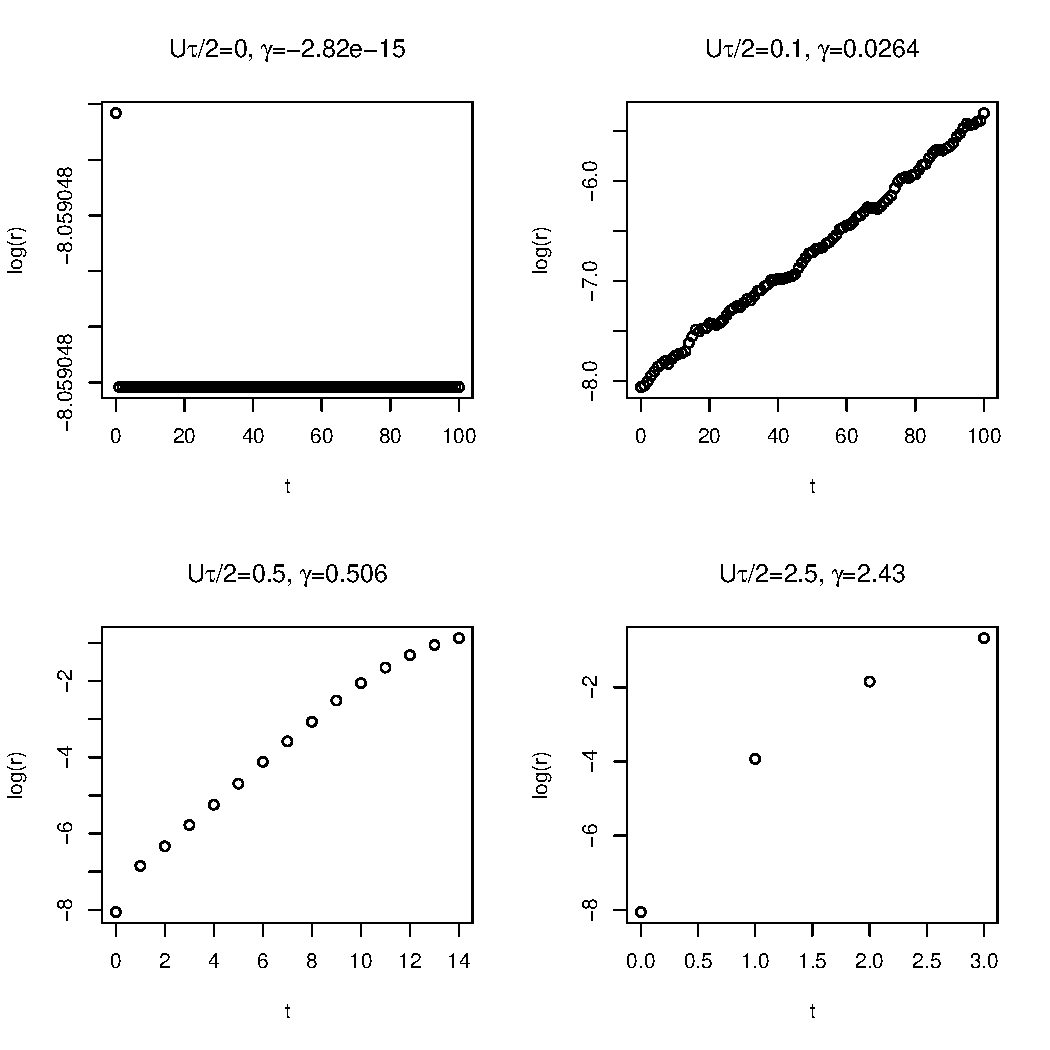
\includegraphics[width=0.875\textwidth]{../code/figure/gamma_for_different_Utot.pdf}
\par\end{centering}
\caption{Estimates of $\gamma$ for different $U\tau/2$.\label{fig:gamma_Utot}}
\end{figure}

